\subsection{Use cases}\label{ssc:usecases}
Below, the use cases from the actor table (see \autoref{tab:actor_table}), have been described. The description includes how the interactions with the system will take place, which actors are involved, and which functions are called, within the system, to complete the actions in the use cases.
\par
Each use case has been described and is followed by a diagram of the interaction.
% In the system definition it was stated that the admin should be able to print out a report of assets from the system. The report will consist of a number of assets, and take shape as a file, saved on the admins computer.
\newpage

\fancyLayout{use_case}{Add an asset}
    {Use case for adding an asset}
    {use_case:add_an_asset}
    {
        \textbf{Use Case:} Adding an asset is done by the admin. An admin goes to the add asset page and fills in all the information about the asset, including the location of the asset and which department it belongs to. After all the information has been added to the asset, the asset is saved in the system and is visible to all employees and can be loaned out.
    
        \vskip 0.2cm
        
        \textbf{Objects:} Admin, Asset
        
        \vskip 0.2cm
        
        \textbf{Functions:} Add asset
    }

\begin{figure}[H]
    \centering
    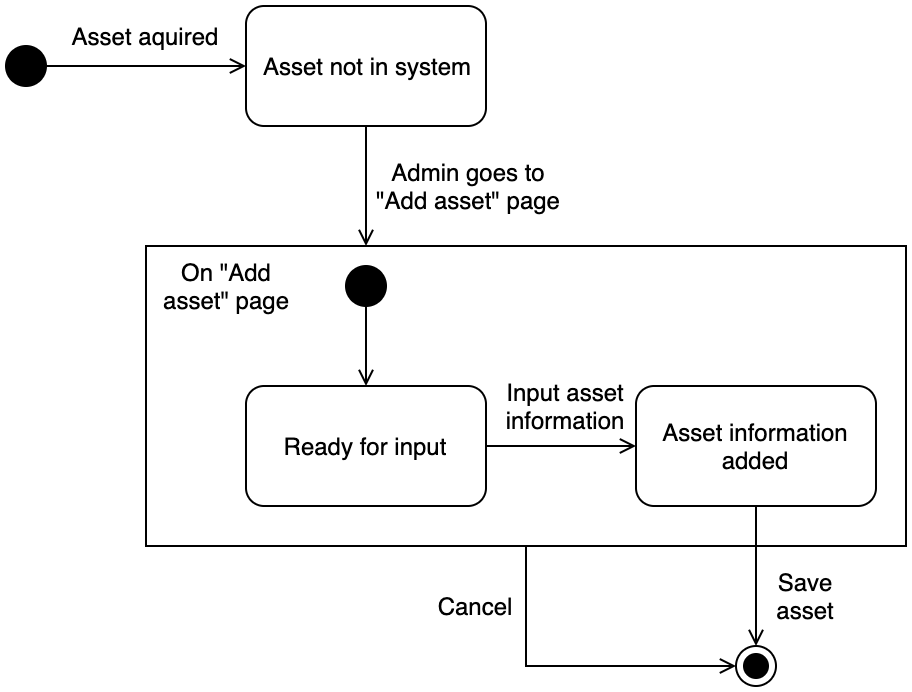
\includegraphics[width=0.8\textwidth]{figures/UC_Add_asset.png}
    \caption{User interface state chart diagram for adding an asset}
    \label{fig:add_asset_statechart}
\end{figure}

\newpage

\fancyLayout{use_case}{Loan out an asset}
    {Use case for loaning out an asset}
    {use_case:loan_out_an_asset}
    {
        \textbf{Use Case:} Loaning out an asset is being carried out by an admin, whom an employee contacts, when they want to borrow the given asset. The admin goes to the page of the given asset and changes its state to loaned out, as well as its location.
    
        \vskip 0.2cm
        
        \textbf{Objects:} Admin, Asset, Employee
        
        \vskip 0.2cm
        
        \textbf{Functions:} Update asset information
    }
 
\begin{figure}[H]
    \centering
    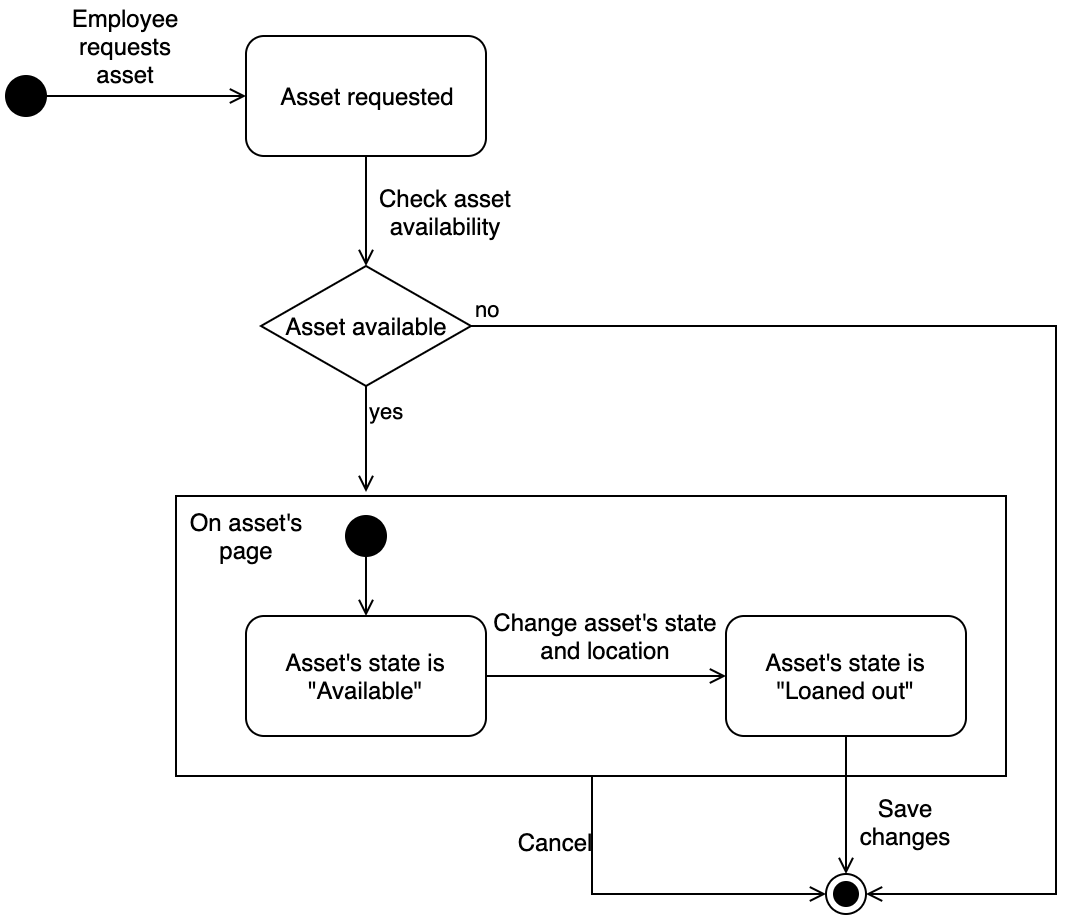
\includegraphics[width=0.8\textwidth]{figures/UC_Loan_out_asset.png}
    \caption{User interface state chart diagram for loaning out an asset}
    \label{fig:loan_out_asse_statechart}
\end{figure}
 
 \newpage
 
\fancyLayout{use_case}{Return an asset}
    {Use case for returning an asset}
    {use_case:return_an_asset}
    {
        \textbf{Use Case:} When an asset is being returned by an employee, it is given to an admin. The admin then goes to the page of the given asset and updates the location and status of the asset.
    
        \vskip 0.2cm
        
        \textbf{Objects:} Admin, Asset, Employee
        
        \vskip 0.2cm
        
        \textbf{Functions:} Update asset information
    }
    
\begin{figure}[H]
    \centering
    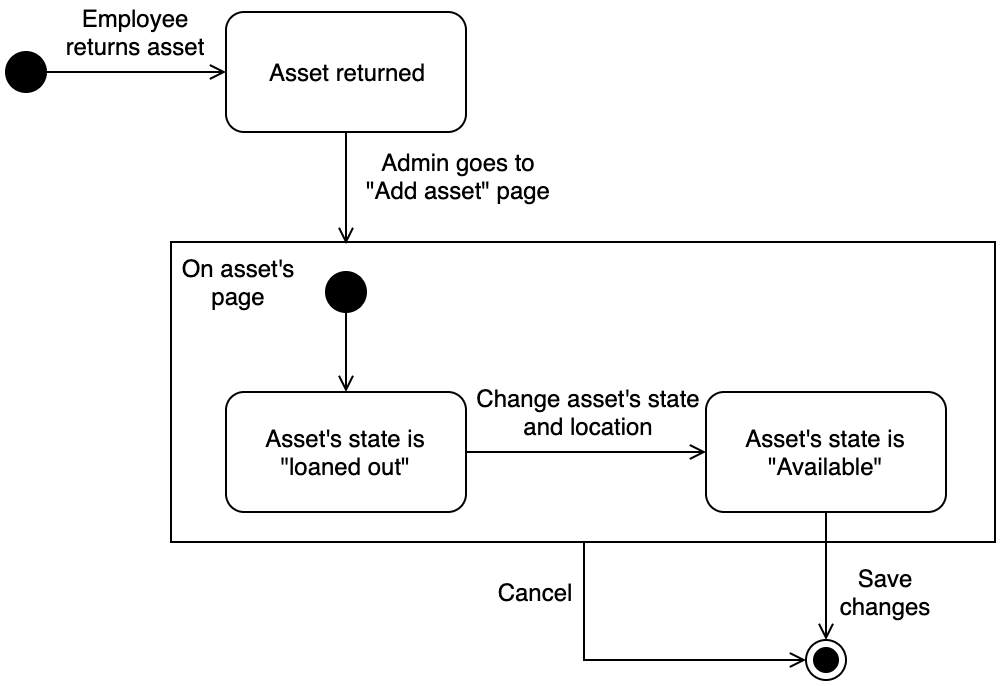
\includegraphics[width=0.8\textwidth]{figures/UC_Return_asset.png}
    \caption{User interface state chart diagram for returning an asset}
    \label{fig:return_asset_statechart}
\end{figure}

\newpage

\fancyLayout{use_case}{Change the information about an asset}
    {Use case for changing the information about an asset}
    {use_case:changing_the_information_about_an_asset}
    {
        \textbf{Use Case:} If one of the states of an asset changes, these changes should be updated in the system by an admin. These state changes could be things such as the asset going from working to being broken, or being updated to a new operation system. To update the asset's information, the admin goes to the given asset's page, potentially through the search page. The admin can then press the edit button and change the outdated data to comply to the new state of the asset in the problem domain.
    
        \vskip 0.2cm
        
        \textbf{Objects:} Admin, Asset
        
        \vskip 0.2cm
        
        \textbf{Functions:} Search for asset, Update asset information, View asset
    }
    
\begin{figure}[H]
    \centering
    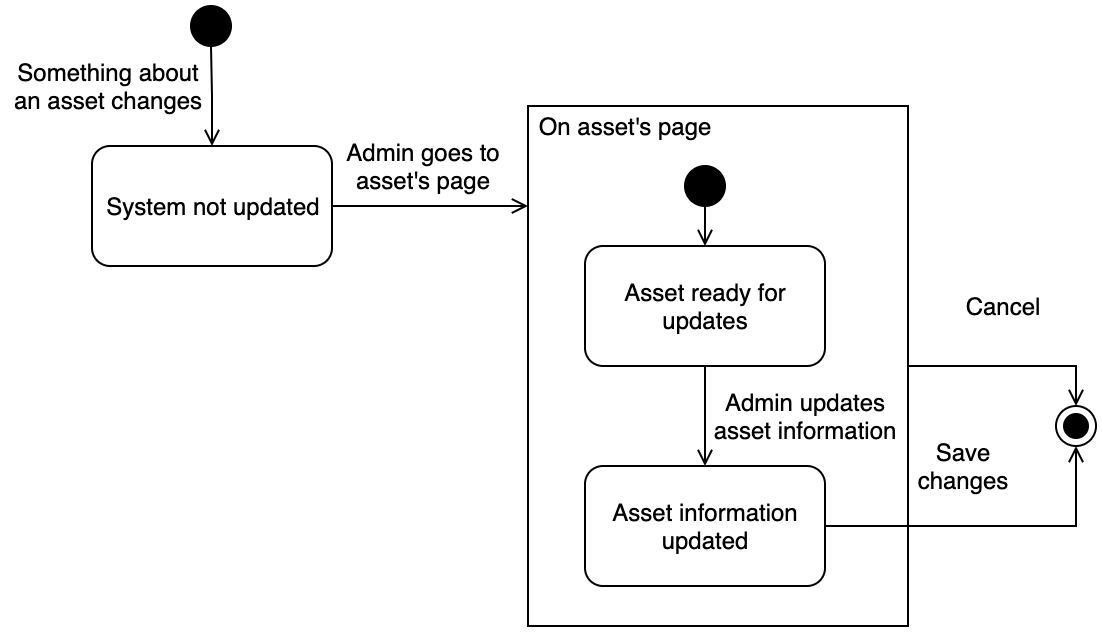
\includegraphics[width=0.8\textwidth]{figures/UC_Change_asset.png}
    \caption{User interface state chart diagram for changing an asset}
    \label{fig:edit_asset_statechart}
\end{figure}

\newpage

\fancyLayout{use_case}{Remove an asset}
    {Use case for removing an asset}
    {use_case:remove_an_asset}
    {
        \textbf{Use Case:} When an asset is no longer needed within the problem domain, it is discarded. This is handled in the system by an admin. The admin goes to the page of the given asset and deletes it from the system. The asset is then removed from the system and is no longer visible to any of the employees.
    
        \vskip 0.2cm
        
        \textbf{Objects:} Admin, Asset, Employee
        
        \vskip 0.2cm
        
        \textbf{Functions:} Remove asset
    }

\begin{figure}[H]
    \centering
    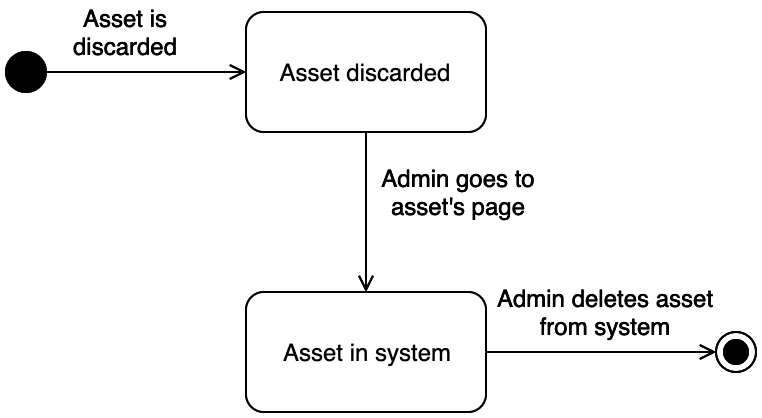
\includegraphics[width=0.8\textwidth]{figures/UC_Remove_asset.png}
    \caption{User interface state chart diagram for removing an asset}
    \label{fig:remove_asset_statechart}
\end{figure}

\newpage

\fancyLayout{use_case}{Search for an asset}
    {Use case for searching for an asset}
    {use_case:search_for_an_asset}
    {
        \textbf{Use Case:} If an employee needs to know something about an asset, the employee goes to the search page, chooses a department and enters in some information about the asset in the search field. The system then returns a list of assets complying with the search query. The employee can then chose an asset and go to its page.
    
        \vskip 0.2cm
        
        \textbf{Objects:} Asset, Employee
        
        \vskip 0.2cm
        
        \textbf{Functions:} Search for asset, View asset
    }

\begin{figure}[H]
    \centering
    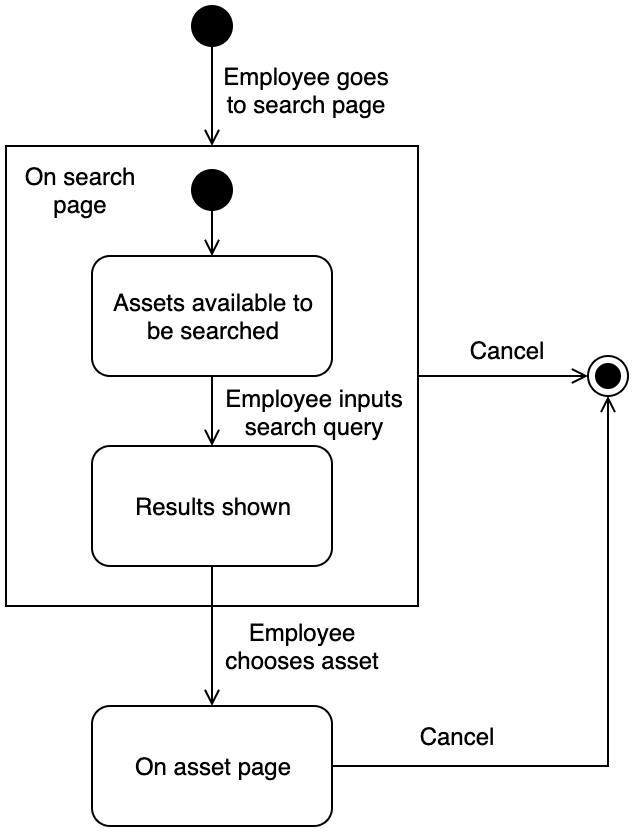
\includegraphics[width=0.6\textwidth]{figures/UC_Search_asset.png}
    \caption{User interface state chart diagram for searching for an asset}
    \label{fig:search_asset_statechart}
\end{figure}

\newpage

\fancyLayout{use_case}{Print a report of assets}
    {Use case for printing a report of assets}
    {use_case:print_a_report_of_assets}
    {
        \textbf{Use Case:} As the number of assets increase in the system, an admin might want to retrieve a number of assets to see outside of the system. The admin goes to the search page and enters a search query, which the assets they want to retrieve from the system must comply with. The admin then selects a number of assets and presses the print button. The system then creates a document containing information about the selected assets and saves it on the admins computer.
    
        \vskip 0.2cm
        
        \textbf{Objects:} Admin, Asset
        
        \vskip 0.2cm
        
        \textbf{Functions:} Export report, Search of asset
    }

\begin{figure}[H]
    \centering
    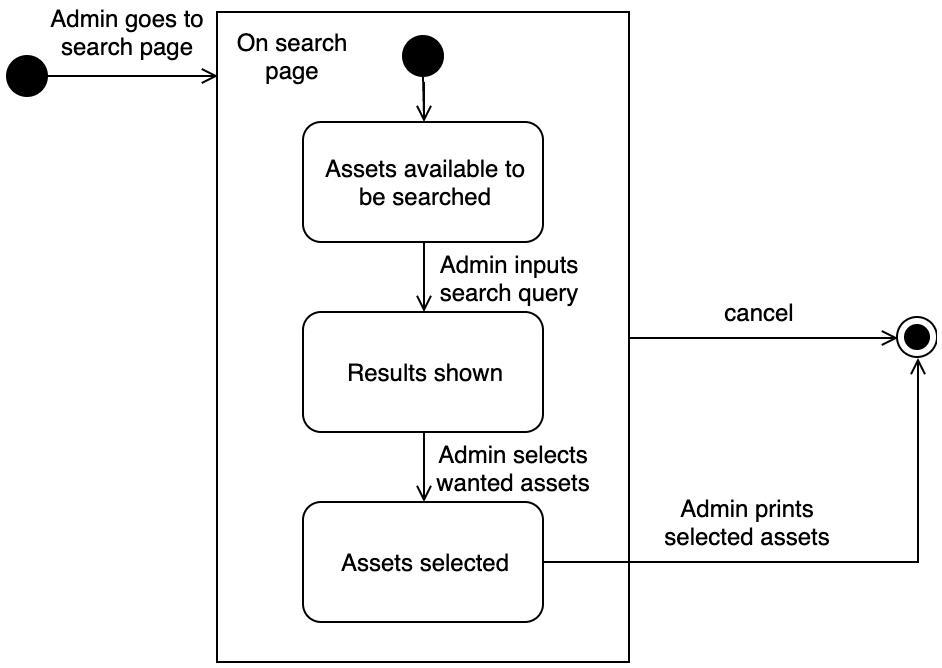
\includegraphics[width=0.8\textwidth]{figures/UC_Print_report.png}
    \caption{User interface state chart diagram for printing out a report}
    \label{fig:print_report_statechart}
\end{figure}

\newpage

\fancyLayout{use_case}{Comment an asset}
    {Use case for commenting on an asset}
    {use_case:commenting_on_an_asset}
    {
        \textbf{Use Case:} An employee might have a comment regarding an asset they have borrowed, such as an issue they had with it or suggestions for improvements. They can then go to the assets page and add a comment to it. This comment will be visible to the admin. 
    
        \vskip 0.2cm
        
        \textbf{Objects:} Employee, Asset, Admin
        
        \vskip 0.2cm
        
        \textbf{Functions:} Search for asset, Add comment to asset
    }

\begin{figure}[H]
    \centering
    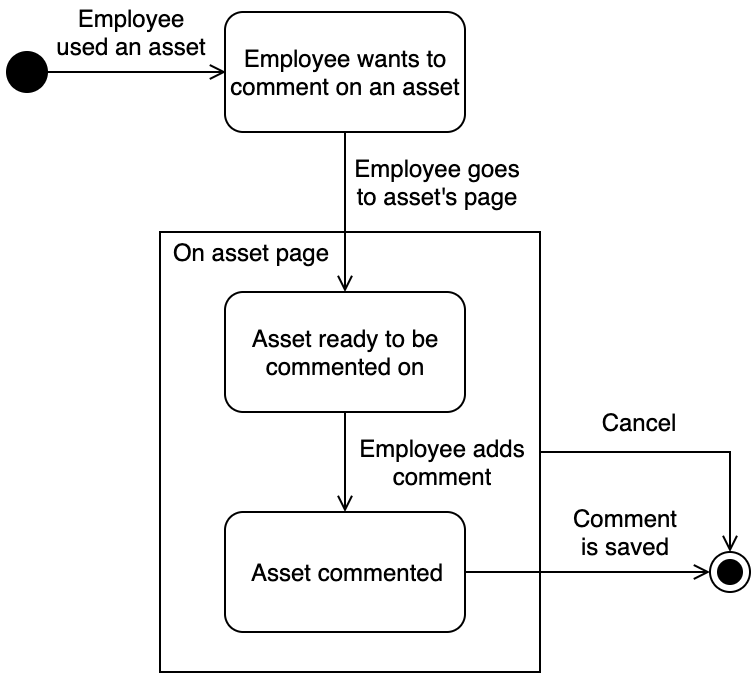
\includegraphics[width=0.8\textwidth]{figures/UC_Add_comment.png}
    \caption{User interface state chart diagram for adding a comment to an asset}
    \label{fig:add_comment_statechart}
\end{figure}

\par
Based on the system definition and requirements, the use cases have been constructed (see \autoref{tab:actor_table}). These are the relevant use cases to handle the assets.

\begin{table}[H]
    \centering
    % \hrule
    \vspace{0.2cm}
    \hspace{6cm} \vspace{0.6cm} \textbf{Actors}
    \begin{tabular}{p{0.5\textwidth} || p{0.2\textwidth} p{0.2\textwidth}}
        \textbf{Use cases} & Admin & Employee \vspace{0.2cm}\\
        \hline \hline
        Add an asset & \hspace{0.34cm} \checkmark & \\
        \hline
        Loan out an asset & \hspace{0.34cm} \checkmark & \hspace{0.6cm} \checkmark \\
        \hline
        Return an asset & \hspace{0.34cm} \checkmark & \hspace{0.6cm} \checkmark \\
        \hline
        Change the information about an asset & \hspace{0.34cm} \checkmark & \\
        \hline
        Remove an asset & \hspace{0.34cm} \checkmark & \\
        \hline
        Search for an asset & \hspace{0.34cm} \checkmark & \hspace{0.6cm} \checkmark \\
        \hline
        Print a report of assets & \hspace{0.34cm} \checkmark & \\
        \hline
        Comment an asset & \hspace{0.34cm} \checkmark & \\
    \end{tabular}
    \vspace{0.2cm}
    % \hrule
    \vspace{0.2cm}
    \caption{Actor table of the relations between actors and use cases.}
    \label{tab:actor_table}
\end{table}

In the actor table above (see \autoref{tab:actor_table}), it has become clear that the admin takes part in every use case. This can be explained by the way the system will be used. The system should function almost like an interface to a database, so it makes sense that the admin will be involved in all the changes made to the system and, as an effect of this, the database.

\par
The defined use cases have then been used to extract relevant functions and, later in the report, construct the user interface. For most of these use cases, the system desires to know which employee or admin committed the changes to the system, and therefore two more functions are needed. \textit{Authenticate user} and \textit{Check access level} are used to satisfy this desire and is executed on login and most of the described use cases above.